\documentclass{beamer}
\mode<presentation>{\usetheme{Madrid}}

\usepackage[utf8]{inputenc}
\usepackage{varwidth}
% Allows including images.
\usepackage{graphicx}
\setcounter{tocdepth}{2}

\title[Linux containers]{Linux containers}

\author{Bruno Barcarol Guimarães}
\institute[]{\textit{bbgstb@gmail.com}}
\date{2015-07-10}

\begin{document}

\begin{frame}
    \titlepage
\end{frame}

\begin{frame}
    \frametitle{Summary}
    \tableofcontents
\end{frame}

\section{Overview}

\subsection{Technologies}

\begin{frame}
    \frametitle{Container}
    container != vm != lxc != docker
\end{frame}

\begin{frame}
    \frametitle{Container}
    Container
    \begin{itemize}
        \item a process or group of processes
        \item
            executing on the same kernel (\textit{i.e. kernel not virtualized})
        \item
            with different levels of isolation from other processes and kernel
            resources
    \end{itemize}
\end{frame}

\begin{frame}
    \frametitle{Container}
    \centering
    \only<1>{
        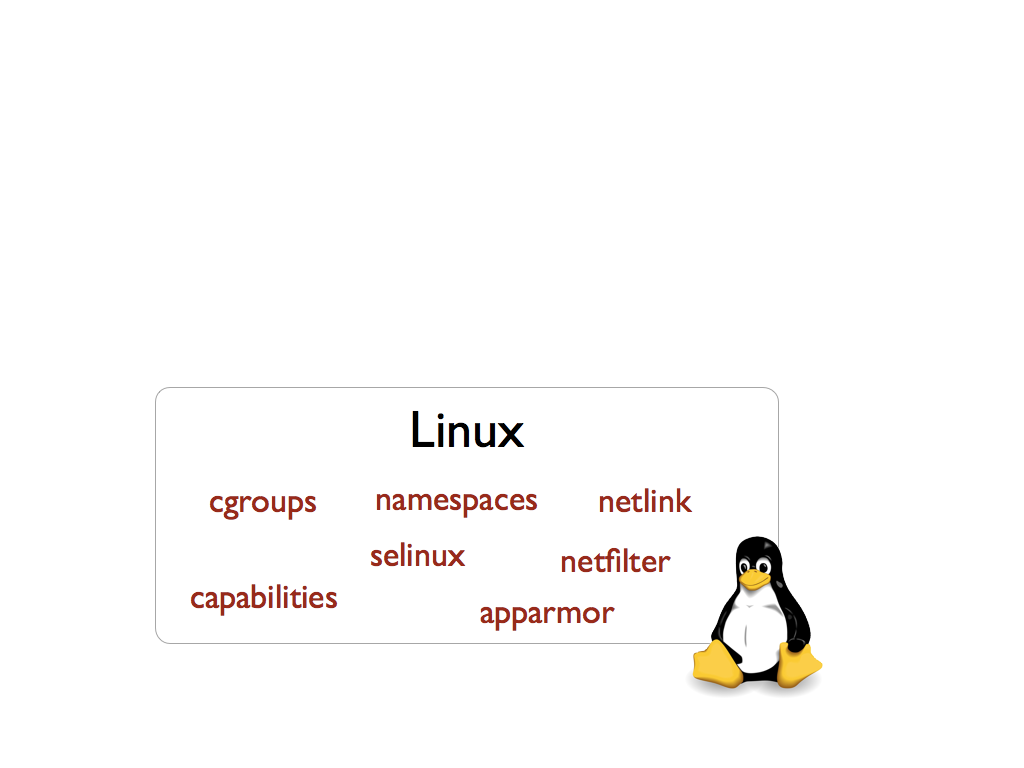
\includegraphics[width=1\linewidth]
            {img/docker_diagram_kernel.png}
    }
    \only<2>{
        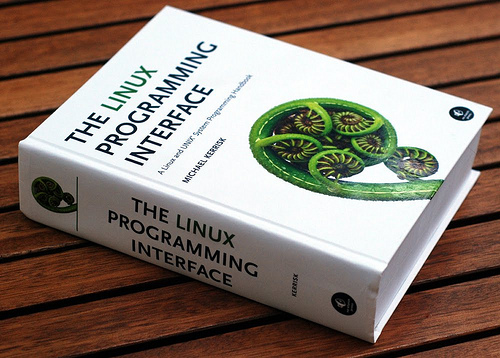
\includegraphics[width=0.8\linewidth]
            {img/the-linux-programming-interface.jpg}
    }
    \only<3>{
        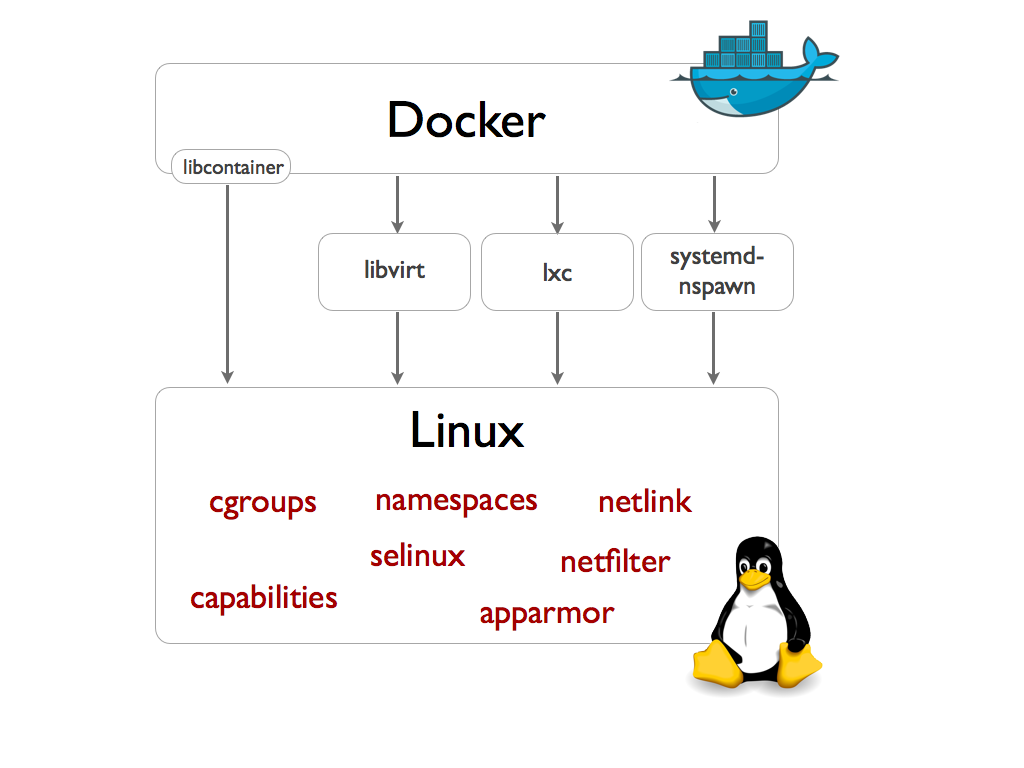
\includegraphics[width=1\linewidth]
            {img/docker-execdriver-diagram.png}
    }
\end{frame}

\subsection{\{A,disa\}dvantages}

\begin{frame}
    \frametitle{Advantages}
    \begin{itemize}
        \item new and highly expanding technologies
        \item shared kernel
            \begin{itemize}
                \item hardware is not virtualized
                \begin{itemize}
                    \item smaller overhead
                    \item smaller resource utilization
                \end{itemize}
                \item faster initialization (\textit{ms})
                \item single update
                    (\textit{kpatch}/\textit{ksplice}/\textit{live patching}?)
            \end{itemize}
    \end{itemize}
\end{frame}

\begin{frame}
    \frametitle{Disadvantages}
    \begin{itemize}
        \item new and highly expanding technologies
        \item shared kernel
        \begin{itemize}
            \item hardware is not virtualized
            \item only one type
            \begin{itemize}
                \item version
                \item architecture
                \item operating system
            \end{itemize}
            \item kernel exploits
        \end{itemize}
    \end{itemize}
\end{frame}

\begin{frame}
    \frametitle{Overview}
    \begin{quote}
        There’s an additional advantage to containerizing your application. It
        forces you to think hard about configuration, limiting the amount of
        mutable state inside your environment and your ability to scale
        horizontally.
        \\~\\
        An exercise in switching to container-based deploys is actually an
        exercise in good engineering practices and any extra work required by
        Docker pays off by making your codebase better factored and less
        brittle.
    \end{quote}
    Jan Urbański - New Relic
\end{frame}

\section{Implementation}

\subsection{kernel}

\begin{frame}
    \frametitle{kernel}
    \begin{itemize}
        \item cgroups
        \item namespaces
    \end{itemize}
\end{frame}

\subsection{cgroups}

\begin{frame}
    \frametitle{cgroups}
    \begin{itemize}
        \item linux 2.6.24 (2007)
        \item resource limiting/reservation
        \item accounting/auditing
    \end{itemize}
\end{frame}

\subsection{namespaces}

\begin{frame}
    \frametitle{namespaces}
    \begin{itemize}
        \only<1>{
            \item \texttt{unshare(2)}
            \item \texttt{clone(2)}
            \item \texttt{setns(2)}
        }
        \only<2>{
            \item mnt (\texttt{CLONE\_NEWNS})
            \item uts (\texttt{CLONE\_NEWUTS})
            \item ipc (\texttt{CLONE\_NEWIPC})
            \item pid (\texttt{CLONE\_NEWPID})
            \item net (\texttt{CLONE\_NEWNET})
            \item uid (\texttt{CLONE\_NEWUSER})
        }
    \end{itemize}
\end{frame}

\begin{frame}
    \frametitle{mount}
    \begin{itemize}
        \item \texttt{CLONE\_NEWNS}
        \item linux 2.4.19 (2002)
        \item \texttt{mount(2)/umount(2)}
        \item different processes have different visions of the file system
        \item ``\texttt{chroot(2)} on steroids''
        \item sharing of mount points
    \end{itemize}
\end{frame}

\begin{frame}
    \frametitle{uts}
    \begin{itemize}
        \item \texttt{CLONE\_NEWUTS}
        \item linux 2.6.19 (2006)
        \item \texttt{uname(2)}
        \item \texttt{sethotname(2)}
        \item \texttt{setdomainname(2)}
    \end{itemize}
\end{frame}

\begin{frame}
    \frametitle{ipc}
    \begin{itemize}
        \item \texttt{CLONE\_NEWIPC}
        \item linux 2.6.19 (2006) / linux 2.6.30 (2009)
        \item \texttt{svipc(7)}/\texttt{mq\_overview(7)}
    \end{itemize}
\end{frame}

\begin{frame}
    \frametitle{pid}
    \begin{itemize}
        \item \texttt{CLONE\_NEWPID}
        \item linux 2.6.24 (2008)
        \item the same pid may appear on different namespaces
        \item processes don't see processes of other namespaces
        \item migration between hosts
        \item multiple pid 1
        \item pid mapping
        \item can be nested
    \end{itemize}
\end{frame}

\begin{frame}
    \frametitle{net}
    \begin{itemize}
        \item \texttt{CLONE\_NEWNET}
        \item linux 2.6.24 (2008)
        \item each namespace has its own
            \begin{itemize}
                \item network devices
                \item ip addresses
                \item routing tables
                \item \texttt{/proc/net}
                \item ports
                \item etc.
            \end{itemize}
    \end{itemize}
\end{frame}

\begin{frame}
    \frametitle{user}
    \begin{itemize}
        \item \texttt{CLONE\_NEWUSER}
        \item linux 2.6.23 (2007)
        \item finalized on kernel 3.8 (2013) $->$ $\sim$ five years
        \item uid and gid isolation and mapping
        \item \texttt{uid 0}
        \item recursive
        \begin{itemize}
            \item an unprivileged process can create a namespace
            \item \texttt{uid 0} inside the namespace
            \item<2> ö
        \end{itemize}
    \end{itemize}
\end{frame}

\begin{frame}[fragile]
    \frametitle{demo}
    \begin{semiverbatim}
        \only<1>{
# create containers
./ns_test
# create pairs of veths
ip link add h1 type veth peer name c1
ip link add h2 type veth peer name c2
# move one to each container's namespace
ip link set dev c1 netns /proc/$pid1/ns/net
ip link set dev c2 netns /proc/$pid2/ns/net
# rename each container's veth to eth0
nsenter --net --target $pid1 ip link set dev c1 name eth0
nsenter --net --target $pid2 ip link set dev c2 name eth0
        }
        \only<2>{
# assign addresses to each container's interfaces
nsenter -n -t $pid1 ip addr add 10.0.0.2/8 dev eth0
nsenter -n -t $pid2 ip addr add 10.0.0.3/8 dev eth0
nsenter -n -t $pid1 ip set eth0 up
nsenter -n -t $pid2 ip set eth0 up
ip link set h1 up
ip link set h2 up
# create a bridge and add the containers' interfaces
brctl addbr br0
brctl addif br0 h1 h2
        }
    \end{semiverbatim}
\end{frame}

\begin{frame}[fragile]
    \frametitle{demo}
    \begin{figure}
        \centering
        \begin{varwidth}{\linewidth}
            \begin{verbatim}
 -- container0 --   -- container1 --
|      eth0      | |      eth0      |
 --------|-------   --------|-------
         |                  |
 --------|------ br0 -------|-------
|        h1                 h2      |
 -----------------------------------
            \end{verbatim}
        \end{varwidth}
    \end{figure}
\end{frame}

\section{Security}

\subsection{uid 0}

\begin{frame}
    \frametitle{uid 0}
    \only<1>{
        \begin{itemize}
            \item don't use
        \end{itemize}
    }
    \only<2>{
        \begin{quote}
            For repos we recognize on or after 2015-01-01, linux builds are
            sent to our container-based infrastructure.
        \end{quote}
        Travis CI
    }
    \only<3>{
        \begin{quote}
            This job is running on container-based infrastructure, which
            does not allow use of 'sudo', setuid and setguid executables.
            If you require sudo, add 'sudo: required' to your .travis.yml
        \end{quote}
        Travis CI
    }
\end{frame}

\subsection{Applications}

\begin{frame}
    \frametitle{Applications}
    \begin{itemize}
        \item
            Most containers execute a specific task, instead of a complete
            system, and most applications (\textit{apache}, \textit{nginx},
            \textit{postgresql}, \textit{redis}, ...) don't need \textit{root}
            privileges.
        \item
            The risks are the same as before: assume the application can do
            anything to escape isolation.
    \end{itemize}
\end{frame}

\begin{frame}
    \frametitle{Applications}
    \only<1>{
        syscalls
        \begin{itemize}
            \item e.g. \texttt{vmsplice(2)}
            \item limits the \textit{syscalls} available
            \item seccomp/seccomp-bpf
            \item \texttt{capabilities(7)}
            \item \texttt{selinux(8)}/\texttt{apparmor(7)}
            \item grsec
            \item constant updates
        \end{itemize}
        = reduce kernel exposure
    }
    \only<2>{
        \begin{quote}
            ``[...] there's maybe marginal increases in practical security for
            certain kinds of deployment, and perhaps marginal decreases for
            others.  We end up coming back to the attack surface, and it seems
            inevitable that that's always going to be larger in container
            environments. The question is, does it matter? If the larger attack
            surface still only results in one more vulnerability per thousand
            years, you probably don't care. The aim isn't to get containers to
            the same level of security as hypervisors, it's to get them close
            enough that the difference doesn't matter.''
        \end{quote}
        Matthew Garrett
    }
\end{frame}

\section{References}

\begin{frame}
    \frametitle{References}
    \begin{itemize}
        \item
            \href
                {https://blog.newrelic.com/2015/06/18/zero-to-docker/}
                {Zero to docker}
        \item
            \href
                {https://www.kernel.org/doc/Documentation/cgroups-v1/}
                {cgroups docs}
        \item
            \href
                {https://www.kernel.org/doc/Documentation/cgroups-v2.txt}
                {cgroups-v2 docs}
        \item
            \href
                {https://lwn.net/Articles/531114/}
                {Namespaces in operation}
        \item
            \href
                {http://mjg59.dreamwidth.org/33170.html}
                {Linux Container Security}
        \item
            \href
                {http://www.slideshare.net/jpetazzo/docker-linux-containers-lxc-and-security}
                {Docker, Linux Containers (LXC), and security}
        \item
            \href
                {https://lwn.net/Articles/268783/}
                {vmsplice(): the making of a local root exploit}
    \end{itemize}
\end{frame}

\begin{frame}
    \frametitle{References (images)}
    \begin{itemize}
        \item
            \href
                {http://www.servicioswebgratis.com/wp-content/uploads/2012/08/the-linux-programming-interface.jpg}
                {The Linux Programming Interface}
        \item
            \href
                {http://blog.docker.com/2014/03/docker-0-9-introducing-execution-drivers-and-libcontainer/}
                {Docker drivers}
    \end{itemize}
\end{frame}

\end{document}
